%!TEX root = ../main.tex
\doublespacing
\chapter{Future Work and Conclusions}
\label{chap:future}
The principle goals of this thesis were to observe solar radio emission at the highest temporal, spectral and spatial resolutions to date. In order to do this, the REAL-time Transient Acquisition backend was developed and installed at I-LOFAR to record the raw voltages fron the station at their native $5.12 \mu$s temporal resolution.
Secondly, a new technique was implemented for the first time to directly measure the size of radio bursts from their interferometric visibilities. This technique was utilised to determine the size and shape of 30 Type III bursts and to compare this with predictions from modern scattering simulations.
This chapter highlights the next steps that can be taken to advance the knowledge of radio wave generation and propagation in the solar corona even further. I discuss the possibility of observing radio bursts with 5 ns temporal resolution using the Transient Buffer Boards from I-LOFAR. I also outline further work that should be done to fully tie together modern observations and computer simulations and the need for a statistical analysis of Type III and Type IIIb radio bursts in order to bring them in line under the most recent theory of Langmuir wave generation. I then draw this thesis to a close with some concluding remarks.

\section{Primary Scientific Objectives}
The research which has been presented in this thesis has contributed to our knowledge of solar radio emission at low frequencies. WOrk undertaken during this thesis has also resulted in a new facility to record and analyse radio emission using I-LOFAR and a new technique for measuring burst sizes from complex visibility data.
\subsection{Observing Radio Bursts at the Highest Temporal Resolutions.}
Chapter \ref{chap:instrumentation} outlines the development of REALTA, a computing backend for I-LOFAR
\subsection{Observing Radio Bursts at the Highest Spatial Resolutions.}
In Chapter \ref{chap:measuring_source_sizes} I described a new method for determining the size of Type III radio bursts from LOFAR visibilities. Using this I was able to determine the size of a Type IIIb burst to be much beigger than expected from back of the envelope estimates.
\subsection{Comparing Observations of Radio Bursts to Computational Simulations.}
Chapter \ref{chap:observations_vs_theory} discusses the measured similarities and discrepancies between observations of Type III bursts and computer simulations of scattering.
\section{Future Work}
The research outlined in this thesis has laid the path for conntinued development. I dive some examples of what's next here.
\subsection{On Observing Radio Bursts with TBBs}
One of the greatest, unexplored potentials of solar radio astronomy is extremely high temporal resolution of radio bursts. The LOFAR TBBs are capable of recording 5 seconds of raw sampled data from the antennas at its native 5 ns temporal resolution. The TBBs are an extremely powerful tool that allow you to recreate the LFOAR data processing pipeline entirely in software. While this might sound like a nightmare, a young na\"ive Pearse Murphy thought it sounded pretty cool and dedicated too much time to trying them out. Unfortunately, this was during the depths of solar minimum with a radio burst once every few months and as such any data taken was essentially noise. Figure \ref{fig:TBB_timeseries} shows 10 ms of noise recorded by the TBBs from I-LOFAR.
%
%\begin{figure}[ht]
%\centering
%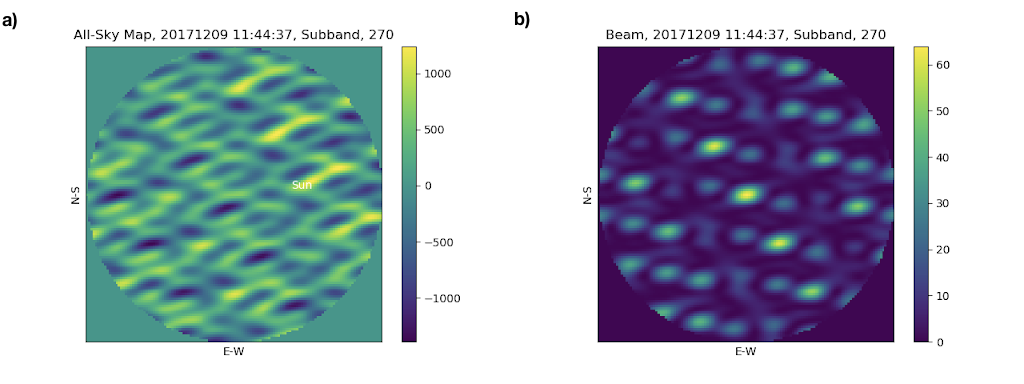
\includegraphics[width=\columnwidth]{AllSky_psf.png}
%\caption[An all sky image made with data from the TBBs at I-LOFAR]{a) An all sky image made with data from the TBBs at I-LOFAR at 52.73 MHz. b) The psf of the antennas for which TBB data was available.}
%\label{fig:TBB_allsky}
%\end{figure}
\begin{figure}[ht]
\centering
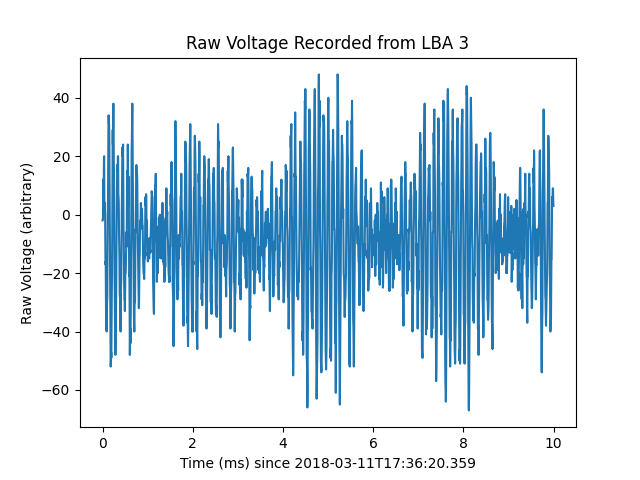
\includegraphics[width=\columnwidth]{TBBtimeseries.png}
\caption[10 ms of data recorded with TBBs from I-LOFAR.]{10 ms of data recorded with TBBs from I-LOFAR, the data presented here is from LBA 3.}
\label{fig:TBB_timeseries}
\end{figure}
\subsection{On Calibrating Solar Interferometric Visibilities}
Interferometric visibilities require calibration in order to account for the effects of the ionosphere. During bursty periods, this calibration can break down and as such more work is needed for a robust calibration procedure for LOFAR.
\subsection{On Automatically Classifying Radio Bursts}
\cite{Scully2021} recently showed promising results of using a convolutional neural network to automatically detect and characterise Type II and Type III radio bursts.

\begin{figure}
\centering
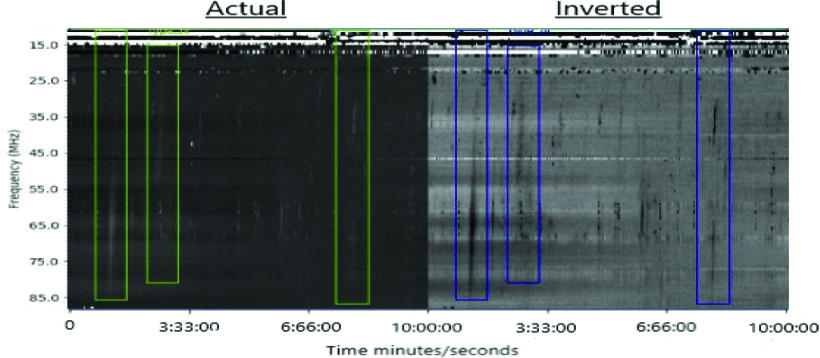
\includegraphics[width=\columnwidth]{scully_yolo.png}
\caption{Automatically detected Type III bursts using YOLO from \cite{Scully2021}
\label{fig:yolo}
\end{figure}
\subsection{On the Statistical Comparisons of Type III and Type IIIb radio bursts}
\cite{Reid2021} presented a theory on Langmuir waves TYpe III and Type IIIb 
\section{Concluding Remarks}
